\documentclass{beamer}
\usepackage[utf8]{inputenc}
\usepackage{graphicx}
\usepackage{fancyvrb}
\usepackage{listings}
\usepackage{eurosym}
\usepackage{xcolor}
\usepackage{textcomp}
\usepackage[ruled, lined]{algorithm2e}
\usetheme{simple}

\let\Tiny=\tiny

\newcommand{\mytilde}{$\sim$}

\definecolor{links}{HTML}{2A1B81}
\hypersetup{colorlinks,linkcolor=,urlcolor=links}

\addtolength{\jot}{0.6em}  % extra space between align rows
\DeclareUnicodeCharacter{20AC}{\euro}

\newcommand{\Xbf}{\ensuremath{\mathbf{X}}}
\newcommand{\xbf}{\ensuremath{\mathbf{x}}}
\newcommand{\wbf}{\ensuremath{\mathbf{w}}}
\newcommand{\ybf}{\ensuremath{\mathbf{y}}}
\newcommand{\epbf}{\ensuremath{\boldsymbol{\epsilon}}}
\newcommand{\Rbb}{\ensuremath{\mathbb{R}}}
\newcommand{\Ebb}{\ensuremath{\mathbb{E}}}

\DeclareMathOperator*{\argmin}{arg\,min}

\usepackage{tikz}
\usetikzlibrary{arrows,shapes,positioning}

\usepackage{multirow}
\usepackage{booktabs}

\graphicspath{{./img/}}

\newenvironment{wideitemize}{\itemize\addtolength{\itemsep}{12pt}}{\enditemize}

\title{Introducción al Data Science}
\author{Alberto Torres Barrán}
\date{3 de Enero del 2020}

%\usepackage{Sweave}
\begin{document}

%% Titulo
\begin{frame}[plain]
\titlepage
\end{frame}

%\begin{frame}
%	\frametitle{Índice}
%    \tableofcontents
%\end{frame}
%
%\AtBeginSection[]
%{
%   \begin{frame}
%       \frametitle{Índice}
%       \tableofcontents[currentsection]
%   \end{frame}
%}

\section{Introducción}

%\begin{frame}
%\frametitle{¿Qué es el ``Big Data''?}
%
%\begin{itemize}
%\item Muchas opiniones, sin una definición clara.
%
%\item En ocasiones se trata simplemente de un término de marketing.
%
%\item A menudo se habla de ``Big Data'' cuando en realidad se hace referencia al \textit{pipeline} de preproceso -- modelado -- visualización y análisis.
%
%\item Los problemas que se resuelven llevan preocupando a los estadísticos unos 50 años, pero en la última década:
%\begin{itemize}
%\item los datos disponibles para analizar han crecido exponencialmente (sociales, sensores, video, imágenes, ...).
%\item han aparecido herramientas que hacen posible análisis de \textbf{grandes} bases de datos.
%\end{itemize}
%\end{itemize}
%\end{frame}
%
%\begin{frame}
%\frametitle{¿Cuanto es \textbf{grande}?}
%
%Según Hadley Wickham (\href{https://www.fields.utoronto.ca/programs/scientific/14-15/bigdata/visualization/hw.pdf}{\textit{Big Data Pipelines}}, Febrero 2015), con la capacidad de computación actual:
%
%\begin{itemize}
%\item Big Data: Can't fit in memory on one computer: $>$ 1 TB
%\item Medium Data: Fits in memory on a server: 10 GB -- 1 TB
%\item Small Data: Fits in memory on a laptop: $<$ 10 GB
%\end{itemize}
%
%Sin embargo, también habla del llamado ``espejismo del Big Data'':
%\begin{itemize}
%\item 90\% Can be reduced to a small/medium data problem with subsetting/sampling/summarising
%\item 9\% Can be reduced to a very large number of small data problems
%\item 1\% Is irreducibly big
%\end{itemize}
%\end{frame}
%
%\begin{frame}[plain]
%\centering
%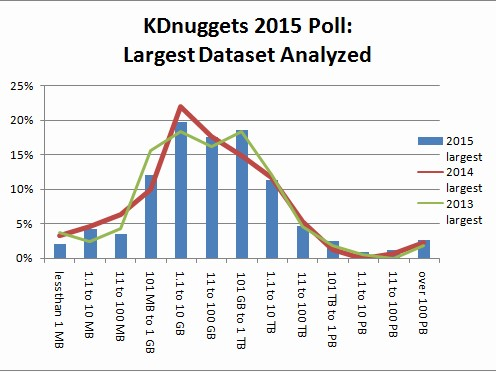
\includegraphics[width=\textwidth]{largest_dataset.jpg}
%{\footnotesize Encuesta: \textit{What was the largest dataset you analyzed?} \href{http://www.kdnuggets.com/2015/08/largest-dataset-analyzed-more-gigabytes-petabytes.html}{Fuente}}
%\end{frame}

\begin{frame}
\frametitle{¿Qué es el \textit{Machine Learning}?}

De la Wikipedia:
\begin{quote}
Machine learning is a subfield of \textbf{computer science} that evolved from the study of \textbf{pattern recognition} and computational learning theory in \textbf{artificial intelligence}.
In 1959, Arthur Samuel defined machine learning as a ``Field of study that gives \textbf{computers the ability to learn without being explicitly programmed}". Machine learning explores the study and construction of algorithms that can learn from and make predictions on data.
\end{quote}

Está íntimamente ligado con otras disciplinas.
\end{frame}

\begin{frame}[plain]
\begin{center}
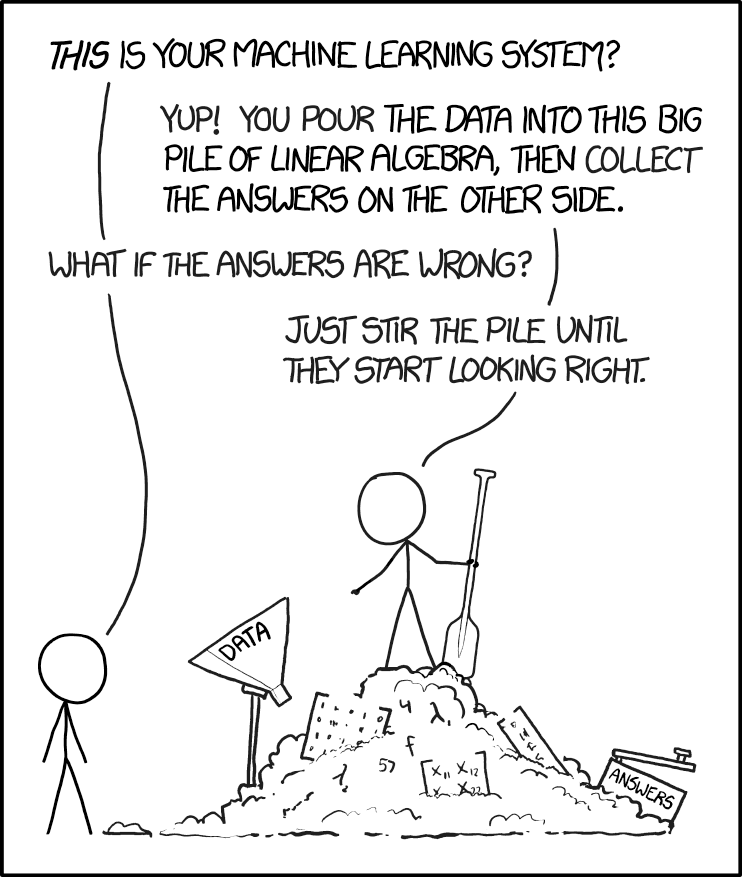
\includegraphics[height=0.85\textheight]{machine_learning_2x.png}

{\footnotesize \href{https://xkcd.com/1838/}{Fuente}}
\end{center}
\end{frame}

\begin{frame}[plain]
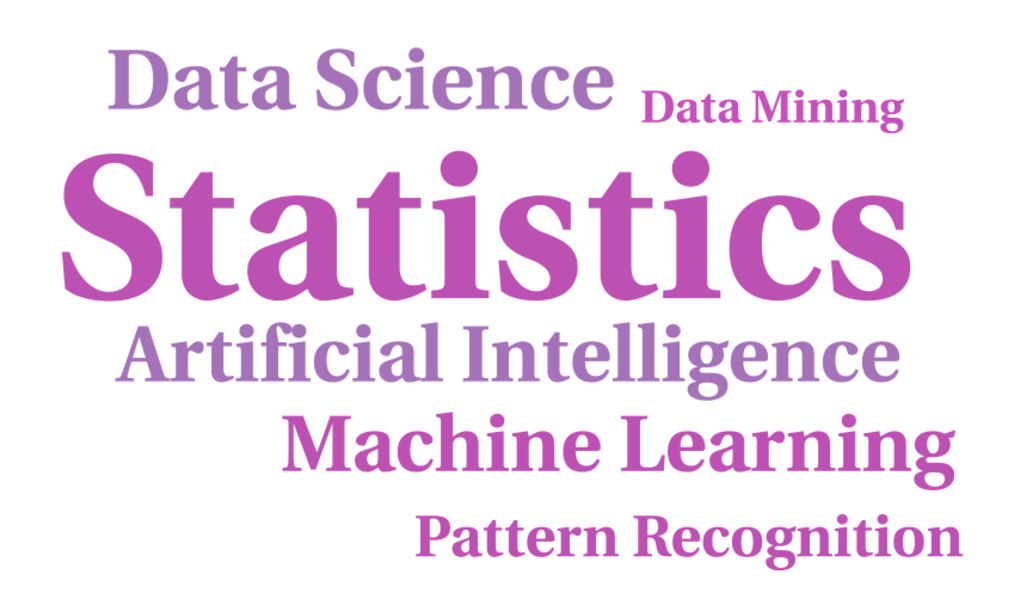
\includegraphics[width=\textwidth]{cloud.pdf}
\end{frame}

\begin{frame}[plain]
\begin{description}
\item[Statistics] Más antigua (aprox. 1749), el resto de disciplinas utilizan algunas de sus técnicas: estadística descriptiva, análisis de regresión, inferencia.
\item[Artificial Intelligence] Más moderna, 1940. Algunos problemas que intenta resolver: procesamiento lenguaje natural, planificación, visión por computador, robótica.
\item[Machine Learning] Rama de la IA, 1946. Se utiliza para resolver algunos de los problemas que tiene la IA.
\item[Pattern Recognition] En general se usa como sinónimo de \textit{Machine Learning}.
\item[Data Mining] Técnicas de modelado estadístico y \textit{machine learning} aplicadas a un dominio en concreto.
\item[Data Science] Término más moderno, mezcla de todo lo anterior.
\end{description}
\end{frame}

\begin{frame}
\frametitle{\textit{Data scientist}}

De la Wikipedia:
\begin{quote}
Data science employs techniques and theories drawn from many fields within the broad areas of mathematics, statistics, information science, and computer science, including signal processing, probability models, machine learning, statistical learning, data mining, database, data engineering, pattern recognition and learning, visualization, predictive analytics, uncertainty modeling, data warehousing, data compression, computer programming, artificial intelligence, and high performance computing.
\end{quote}

La conclusión es que se tratan de un perfil muy amplio, con un conjunto de habilidades poco definido.
\end{frame}


\begin{frame}
\frametitle{\textit{Data science} en la empresa}
\begin{itemize}
\item En 2012, Harvard Business Review publicó el artículo:

\begin{center}
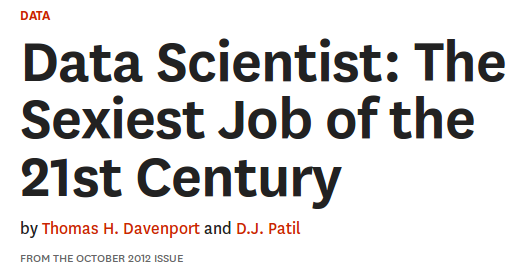
\includegraphics[scale=0.4]{data.png}
\end{center}

\item La consultora \href{http://www.mckinsey.com/business-functions/business-technology/our-insights/big-data-the-next-frontier-for-innovation}{McKinsey} calcula que para 2018 habrá una demanda de entre 140,000-190,000 puestos de \textit{data science} sin cubrir.

\item Nadie sabe muy bien lo que es pero todo el mundo quiere uno.
\end{itemize}
\end{frame}


\begin{frame}
\frametitle{Flujo de trabajo de un equipo de \textit{data science}}
\begin{itemize}
\item En ocasiones un único perfil realiza todas las tareas.
\item Sin embargo, cada vez es más habitual tener un equipo donde cada integrante esté especializado en distintas partes del proceso. 
\end{itemize}
\begin{center}
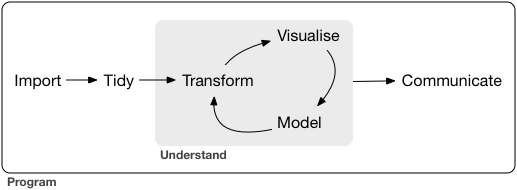
\includegraphics[width=0.85\textwidth]{data-science.png}

{\footnotesize Fuente: Hadley Wickham, \href{http://r4ds.had.co.nz/}{R for Data Science}}
\end{center}
\end{frame}

\begin{frame}[plain]
\frametitle{Herramientas de análisis}

\begin{center}
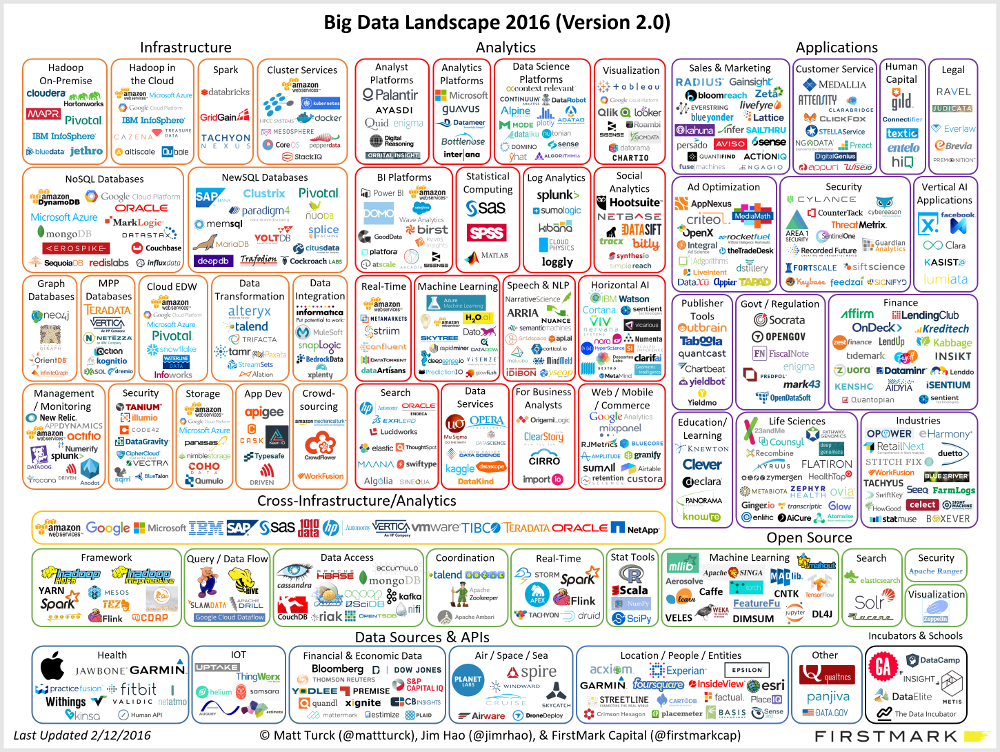
\includegraphics[width=\textwidth]{big_data_landscape.png}
\end{center}
\end{frame}


\begin{frame}[plain]
\begin{center}
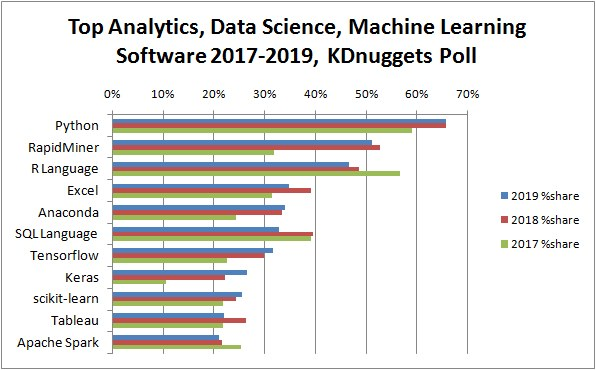
\includegraphics[height=0.75\textheight]{top-analytics-data-science-machine-learning-software-2019-3yrs-590.jpg}
\end{center}
{\footnotesize Software para proyectos de \textit{analytics}, y \textit{data science}. Encuesta de \href{https://www.kdnuggets.com/2019/05/poll-top-data-science-machine-learning-platforms.html}{KDnuggets}.}
\end{frame}


\begin{frame}
\frametitle{Colecciones de paquetes útiles}
\begin{itemize}
\item En \href{https://support.rstudio.com/hc/en-us/articles/201057987-Quick-list-of-useful-R-packages}{este} enlace se puede ver una lista muy reciente de paquetes útiles.
\item \href{https://cran.r-project.org/web/views/MachineLearning.html}{Machine Learning in R} es una colección de paquetes de aprendizaje automático.
\item \href{http://cran.r-project.org/web/views/HighPerformanceComputing.html}{High-Performance computing in R} es una colección de paquetes de útiles para la computación de alto rendimiento.
\item Recientemente aplicaciones web que permiten la visualización de resultados también gozan de gran popularidad, por ejemplo los notebooks de \href{http://jupyter.org/}{Jupyter}.
\item En R destaca \href{http://shiny.rstudio.com/}{Shiny}, que permite convertir código R en aplicaciones web interactivas.
\end{itemize}
\end{frame}

\begin{frame}
\frametitle{Paquetes más populares de ML}
\centering
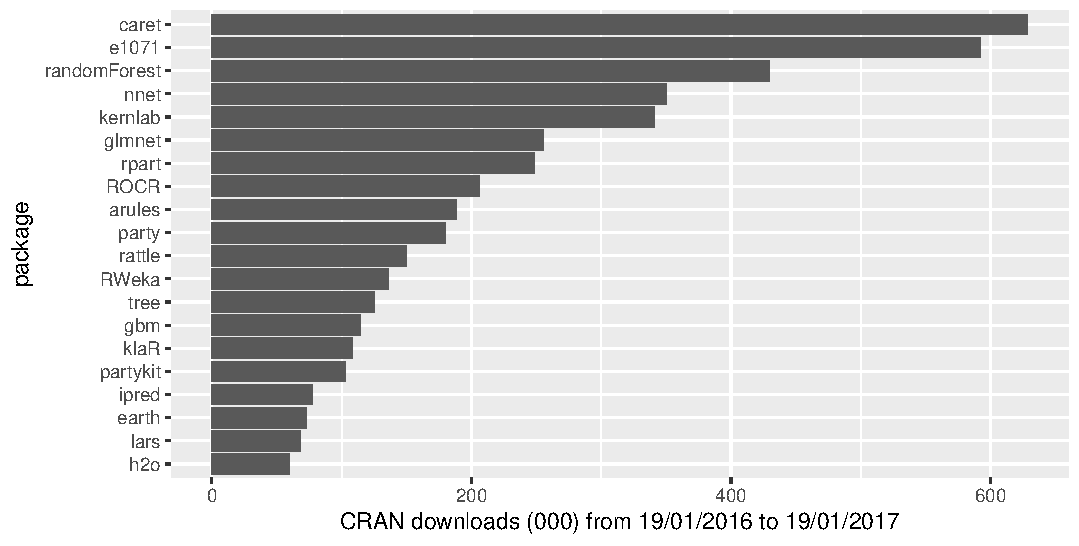
\includegraphics[width=\textwidth]{top20.pdf}

{\footnotesize Descargas Enero 2016 - Enero 2017. \href{https://github.com/thedataincubator/data-science-blogs}{Fuente}}
\end{frame}


\begin{frame}
\frametitle{Resumen paquetes destacados}
\begin{itemize}\addtolength{\itemsep}{0.3\baselineskip}
\item Modelos lineales y utilidades:
\begin{itemize}
\item \texttt{caret}, utilidades para clasificación y regresión
\item \texttt{MASS}, ridge regression
\item \texttt{ridge}, ridge regression con selección automática del hiper-parámetro
\item \texttt{glmnet}, GLMs con regularización Lasso o Elastic Net
\item \texttt{glmnetUtils}, utilidades para \texttt{glmnet}
\item \texttt{gam}, modelos aditivos generalizados
\item \texttt{mgcv}, modelos adictivos generalizados (recomendado)
\end{itemize}
\item Algunos modelos más complejos:
\begin{itemize}
\item \texttt{nnet}, Redes neuronales, también regresión logística multinomial
\item \texttt{e1071}, Support Vector Machines
\item \texttt{gbm}, Gradient Boosting
\item \texttt{randomForest}, Random Forest
\item \texttt{xgboost}, Extreme Gradient Boosting
\end{itemize}
\end{itemize}
\end{frame}


\begin{frame}
\frametitle{\textit{Tidyverse}}

\begin{itemize}
\item Conjunto de paquetes creados por Hadley Wickham que comparten una misma API y contienen funciones para el análisis de datos:
\begin{itemize}
    \item \textbf{\texttt{ggplot2}}, para hacer gráficos avanzados.
    \item \textbf{\texttt{dplyr}}, para manipular datos.
    \item \textbf{\texttt{tidyr}}, para limpiar datos.
    \item \textbf{\texttt{readr}}, para importar datos.
    \item \texttt{purrr}, para programación funcional.
    \item \texttt{tibble}, implementa \textit{tibbles}, una versión moderna de los data.frames.
\end{itemize}

\item El paquete \textit{tidyverse} instala y carga los paquetes anteriores.

\item También instala otros paquetes que pueden ser útiles aunque no los carga por defecto.

\item Para más información y la lista completa de paquetes: \url{https://github.com/tidyverse/tidyverse}.
\end{itemize}
\end{frame}


\begin{frame}
\frametitle{Libros y manuales}

En general, se pueden encontrar muchos manuales en las secciones \textit{Manuals} y \textit{Contributed} de \href{https://cran.r-project.org/}{CRAN}, así como ejemplos en la web \href{https://rpubs.com/}{RPubs}. Algunos recursos más específicos:

\begin{description}
\item[Libros]
\begin{itemize}
 \item R for Data Science \href{http://r4ds.had.co.nz/}{[url]}.
 \item An Introduction to Statistical Learning with Applications in R \href{http://www-bcf.usc.edu/~gareth/ISL/}{[url]}.
\end{itemize}
\item[E-Books]
\begin{itemize}
\item YaRrr! The Pirate's Guide to R \href{http://nathanieldphillips.com/thepiratesguidetor/}{[url]}.
\item The R Inferno \href{http://www.burns-stat.com/pages/Tutor/R_inferno.pdf}{[url]}.
\item R Programming \href{https://en.wikibooks.org/wiki/R_Programming}{[url]}.
\end{itemize}
\item[Blogs]
\begin{itemize}
\item RTutorial \href{http://www.r-tutor.com/}{[url]}.
\item Quick-R \href{http://www.statmethods.net/}{[url]}.
\item RStudio \href{https://blog.rstudio.org/}{[url]}.
\item RBloggers \href{https://www.r-bloggers.com/}{[url]}.
\end{itemize}
\end{description}

\end{frame}

\begin{frame}
\frametitle{FAQs y comunidades}
\begin{itemize}
\item \href{http://stackoverflow.com/questions/tagged/r}{StackOverflow}: las preguntas con el tag R contienen mucha información y problemas resueltos. Además, las nuevas preguntas se responden en cuestión de horas.

\item \href{http://stats.stackexchange.com/}{CrossValidated}: no es una comunidad específica de R (más bien de estadística), pero hay mucha información acerca de cómo realizar procedimientos concretos de análisis de datos y aprendizaje automático en R.

\item \href{https://twitter.com/RLangTip}{@RLangTip}: Twitter que publica consejos y trucos diarios.

\item \href{https://plus.google.com/u/0/communities/115516770321395255377}{R Programming for Data Analysis}: Comunidad de Google+.
\item \href{https://plus.google.com/u/0/communities/117681470673972651781}{Statistics and R}: Otra comunidad de Google+.
\item \href{https://www.linkedin.com/grp/home?gid=77616}{The R Project for Statistical Computing}: Grupo de LinkedIn.
\end{itemize}
\end{frame}

\begin{frame}
\frametitle{Algunas referencias}
\begin{enumerate}
\item Jerome H. Friedman. \textit{Data Mining and Statistics: What's the Connection?} (1998). \href{http://statweb.stanford.edu/~jhf/ftp/dm-stat.pdf}{[url]}
\item Leo Breiman. \textit{Statistical Modeling: The Two Cultures} (2001). \href{http://projecteuclid.org/download/pdf_1/euclid.ss/1009213726}{[url]}
\item Cross Validated.\textit{What is the difference between data mining, statistics, machine learning and AI?} (2010). \href{http://stats.stackexchange.com/questions/5026/what-is-the-difference-between-data-mining-statistics-machine-learning-and-ai}{[url]}
\item Sakthi Dasan Sekar. \textit{What is the difference between Artificial Intelligence, Machine Learning, Statistics, and Data Mining} (2014). \href{http://shakthydoss.com/what-is-the-difference-between-artificial-intelligence-machine-learning-statistics-and-data-mining/}{[url]}.
\item Cross Validated. \textit{What exactly is Big Data?} (2015). \href{http://stats.stackexchange.com/questions/173060/what-exactly-is-big-data}{[url]}
\item David Donoho. \textit{50 years of Data Science} (2015). \href{http://pages.cs.wisc.edu/~anhai/courses/784-fall15/50YearsDataScience.pdf}{[url]}
\end{enumerate}
\end{frame}

\end{document}
